\documentclass[a4paper,french,10pt]{article}
\usepackage{homework}
\usepackage{diagbox}

% change le nom de la table des matières
\addto\captionsfrench{\renewcommand*\contentsname{Sommaire}}

\lstdefinelanguage{R}%
{morekeywords={function,for,in,if,elseif,else,TRUE,FALSE,%
		return, while, diag, sum, sqrt, nrow, ncol, par, plot, cbind, rep, as, survdiff, survreg, ifelse, anova,
		row, names, colnames, mean, data, frame, model, in, list, rexp, rpois, summary,
		matrix, TRUE, FALSE, for, if, else, function, NA, print, survfit, Surv, rho, ggplot},%
	sensitive=true,%
	morecomment=[l]{\#},%
	morestring=[s]{"}{"},%
	morestring=[s]{'}{'},%
}[keywords,comments,strings]%

\lstset{%
	language         = R,
	basicstyle       = \ttfamily,
	keywordstyle     = \bfseries\color{blue},
	stringstyle      = \color{magenta},
	commentstyle     = \color{olive},
	showstringspaces = false,
}

\begin{document}
	
	% Blank out the traditional title page
	\title{\vspace{-1in}} % no title name
	\author{} % no author name
	\date{} % no date listed
	\maketitle % makes this a title page
	
	% Use custom title macro instead
	\usebox{\myReportTitle}
	\vspace{1in} % spacing below title header
	
	% Assignment title
	{\centering \huge \assignmentName \par}
	{\centering \noindent\rule{4in}{0.1pt} \par}
	\vspace{0.05in}
	{\centering \courseCode~: \courseName~ \par}
	{\centering Rédigé le \pubDate\ en \LaTeX \par}
	\vspace{1in}
	
	% Table of Contents
	\tableofcontents
	\newpage
	
	%----------------------------------------------------------------------------------------
	%	EXERCICE 1
	%----------------------------------------------------------------------------------------
	

\section{Introduction}
Dans le cadre de ce projet, nous allons modéliser le comportement extrême des vagues dans le golfe du lion à l'aide des méthodes vue à travers l'unité d'enseignement HAX005X "valeurs extrêmes". D'après la source \cite{golfLion}, le golf s'étale sur 220 kilomètres de la Camargue à la frontière espagnole. La côte, essentiellement sableuse, a été façonnée par la houle (la mer gagnant souvent les terres par élévation du niveau marin) et l'érosion côtière. L'apport de sédiments en provenance des fleuves a également permis de faire avancer le rivage pendant de longues périodes. Des formations de lagunes "comme les graus" (parfois temporaires) ont pu apparaitre et ont permis de faire communiquer les étangs littoraux avec la mer. Le golf du Lion est donc un milieu naturellement dynamique. C'est dans ce contexte que nous étudions le comportement extrême des vagues à cet endroit, de façon univariée dans un premier temps puis de façon bivariée dans un second temps. 

\newpage

\section{L'algorithme EM}
Dans cette section nous allons nous intéresser à l'algorithme EM (Expectation-Maximization) afin d'estimer les paramètres $\mu$ et $\sigma$ d'un mélange gaussien. Nous avons implémenté cet algorithme via la fonction $EM$ (présente dans notre script $R$) en nous aidant de la source \cite{EM_algorithm}. Afin de tester l'efficacité de notre implémentation, nous allons dans un premier temps l'éxecuter sur des données simulées. En effet, dans notre script, nous avons implémenté une autre fonction que nous avons nommé $simulation$. Cette dernière nous permettra de générer de manière aléatoire, un échantillon issu d'un mélange gaussien. Nous décrirons plus en détaille cette fonction, en aval. Dans un second temps, nous exécuterons notre algorithme sur de vraies données afin de voir s'il est robuste. Pour cela nous utiliserons le jeu de données galaxies de la librairie MASS et nous le décrirons ultérieurement.

\subsection{Implémentation de la fonction simulation}
Comme il a été mentionné précédemment nous allons réaliser dans un premier temps une étude sur des données simulées à partir de la fonction $simulation$. Décrivons cette dernière, elle prend en argument:
\begin{itemize}
	\item \textbf{dt\_param:} Le dataframe contenant les paramètres $\alpha$, $\mu$ et $\sigma$
	\item \textbf{n:} La taille de l'échantillon
\end{itemize}
Elle retourne un vecteur de taille $n$ qui sera l'échantillon du mélange gaussien. \\ Regardons un plus en détaille comment a été conçue cette fonction. \\
La partie la plus importante et la plus subtile de ce script est celle dans laquelle nous distribuons aléatoirement les $(X_i)_{i \in 1,\dots,n}$ de l'échantillon de sorte à avoir un bon mélange gaussien. \\
Afin de simplifier les choses, rien de mieux que de prendre un exemple. Dans celui-ci, l'objectif sera de générer un mélange de quatre gaussiennes, ayant pour paramètres respectifs $\theta_1 = (\alpha_1, \mu_1, \sigma_1)$, $\theta_2 = (\alpha_2, \mu_2, \sigma_2)$, $\theta_3 = (\alpha_3, \mu_3, \sigma_3)$ et $\theta_4 = (\alpha_4, \mu_4, \sigma_4)$. \\
Les $(\alpha_j)_{j \in \{1,\dots,4\}}$ étant ici des probabilités, nous avons que:
\[
	\sum_{j=1}^{4} \alpha_{j} = 1
\]
La démarche est la suivante:
\begin{itemize}
	\item Si $Z < \alpha_1$ alors $X \sim \mathcal{N}(\mu_1, \sigma_1)$
	\item Sinon si $\alpha_1 < Z < \alpha_1 + \alpha_2$ alors $X \sim \mathcal{N}(\mu_2, \sigma_2)$
	\item Sinon si $\alpha_1 + \alpha_2 < Z < \alpha_1 + \alpha_2 + \alpha_3$ alors $X \sim \mathcal{N}(\mu_3, \sigma_3)$
	\item Sinon si $\alpha_1 + \alpha_2 + \alpha_3 < Z < \alpha_1 + \alpha_2 + \alpha_3 + \alpha_4$ alors $X \sim \mathcal{N}(\mu_4, \sigma_4)$
\end{itemize}
Notez que notre implémentation marche dans le cas général d'un mélange de J gaussiennes avec $J \in \mathbb{N}^{*}$.

\subsection{Implémentation de la fonction EM}
La fonction $EM$ est sans aucun doute celle la plus importante de cette section, il est donc primordial de la décrire. \\ 
Tout d'abord, pour implémenter cette dernière, nous nous sommes fortement aidés du pseudo-code suivant:

\begin{algorithm}
	\caption{\textbf{L’algorithme EM (Dempster et al., 1977).}}
	\begin{algorithmic}[1]
		\REQUIRE{$N \in \mathbb{N}$, $\widehat{\theta_0} \in \Theta$, un jeu de données $x_1 \dots x_n$;}
		\ENSURE
		\STATE {$k:=1$;}
		\WHILE {$K < N + 1$}
		\STATE {$\text{\textbf{ETAPE E :} \textit{Calculer la fonction }} Q(\theta;\widehat{\theta}_{k-1}) = \frac{1}{n} \sum_{i=1}^{n} \mathbb{E}_{\widehat{\theta}_{k-1}} [log f(X_i,Z_i,\theta)|X_i = x_i]$;}
		\STATE {$\text{\textbf{ETAPE M : }} \widehat{\theta}_k = argmax \hspace{1.5mm} Q(\theta;\widehat{\theta}_{k-1})$;}
		\STATE {$k \leftarrow k+1$;}
		\ENDWHILE
		\RETURN {$\widehat{\theta}_N$;}
	\end{algorithmic}
\end{algorithm}

La fonction $EM$ prend en argument:
\begin{itemize}
	\item data\_init, le dataframe contenant les paramètres initiaux ($\alpha_{init}$, $\mu_{init}$, $\sigma_{init}$)
	\item X, les données (réelles ou simulées) issues d'un mélange gaussien
	\item K le nombre d'itérations souhaitées pour l'algorithme
\end{itemize}  
Elle retourne un dataframe contenant les valeurs des
paramètres estimées par l'algorithme, à savoir $\alpha$, $\mu$ et $\sigma$. \\
Les formules que nous avons utilisé pour calculer l'étape E et M et qui sont présentées ci dessous sont issue de la source \cite{EM_algorithm}.
\begin{itemize}
	\item Lors de l'étape E nous déterminons la probabilité $\mathbb{P}_{\tilde{\theta}}(Z = j| X = X_i)$ via la formule suivante:
	\[
	\mathbb{P}_{\tilde{\theta}}(Z = j| X = X_i) = \frac{\alpha_j \times \gamma_{\mu_j, j_v}}{\sum_{k=1}^{J} \alpha_k \times \gamma_{\mu_k, v_k}}
	\] \\
	\item Lors de l'étape M, nous déterminons les estimateurs du maximum de vraisemblance $(\widehat{\alpha_j}, \widehat{\mu_j}, \widehat{\sigma_j})$ via les formules suivantes:
	\begin{align*}
		\widehat{\alpha_j} &= \displaystyle\frac{1}{n}\sum_{i=1}^n (Z=j|X=X_i) \\
		\widehat{\mu_j} &= \displaystyle\frac{\displaystyle\sum_{i=1}^n X_i (Z=j|X=X_i)}{\displaystyle\sum_{i=1}^n (Z=j|X=X_i)} \\
		\widehat{v_j} &= \displaystyle\frac{\displaystyle\sum_{i=1}^n (X_i -\widehat{\mu_j})^2 (Z=j|X=X_i)}{\displaystyle\sum_{i=1}^n (Z=j|X=X_i)}
	\end{align*} 
\end{itemize}
\vspace{7mm}
Toutefois, il est important de notifier le fait qu'il n'existe pas de convergence de la suite de paramètres établies par l'algorithme EM. En effet, ces derniers peuvent rester bloqués dans des extremas locaux. On comprend donc qu'il est primordial de choisir de bons paramètres initiaux afin de ne pas être confronté à ce problème. Dans la section consacrée à l'étude sur de vraies données, nous expliciterons la procédure qui a été mise en place pour choisir ces paramètres initiaux.

\newpage

\subsection{Étude sur des données simulées}
Cette sous-section sera consacrée à l'étude menée sur des données simulées à partir de notre fonction $simulation$.

\subsubsection{Simulation d'un mélange de deux gaussiennes } 
Nous avons ici décidé de générer un échantillon de taille 100 issu d'un mélange de deux gaussiennes de lois respectives $\mathcal{N}(\mu_1, \sigma_1) = \mathcal{N}(50, 11)$ et $\mathcal{N}(\mu_2, \sigma_2) = \mathcal{N}(220, 50)$.
La densité associée à cet échantillon a été estimée de manière non paramétrique à partir d'une méthode à noyau et elle a été tracée sur la figure \ref{density_sim}.

\begin{figure}[htp] 
	\centering
	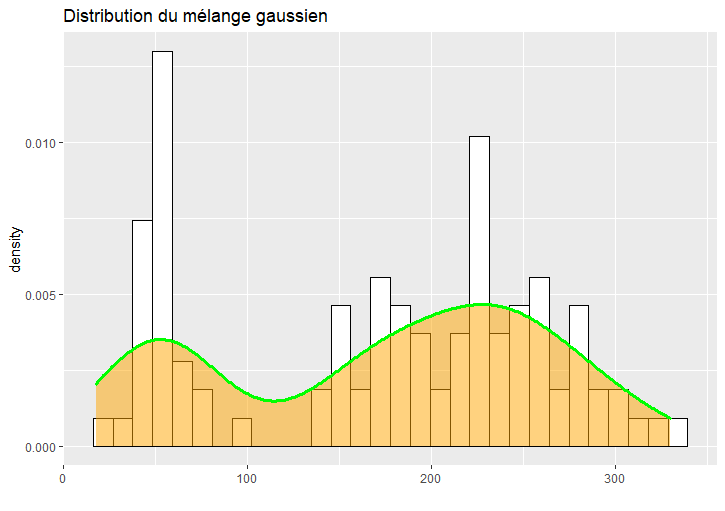
\includegraphics[scale=0.45]{images/dens_sim.png}
	\caption{Densité estimée par méthode à noyau.}
	\label{density_sim}
\end{figure}

Nous avons ensuite appliqué notre algorithme (fonction EM) sur cet échantillon. Le tableau \ref{tab1} contient les valeurs des vrais paramètres de ce mélange simulé. Comme il a été mentionné précédemment, le choix des paramètres initiaux est crucial si l'on veut que l'algorithme estime correctement les paramètres du mélange. Le tableau \ref{tab2} contient les valeurs des paramètres initiaux utilisés. Comme vous pouvez le voir en observant ces deux tableaux, nous avons choisi des paramètre initiaux assez proches des vrais de manière à ne pas être bloqué dans des extremas locaux. Les résultats obtenus par notre algorithme sont affichés sur la capture d'écran de la figure \ref{res_sim}.

 Comme on peut le voir sur la figure \ref{res_sim}, les valeurs estimées par notre implémentation sont proches de celles des vrais paramètres (voir tableau \ref{tab1}). Ces résultats nous montrent donc que notre fonction $EM$ fonctionne correctement, ce qui est rassurant.
 
 \begin{figure}[htp] 
 	\centering
 	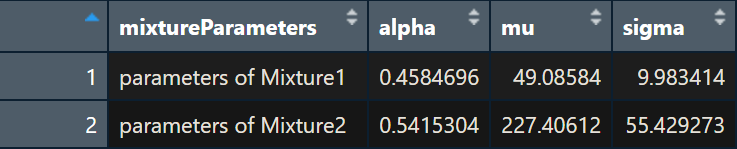
\includegraphics[scale=0.7]{images/res_sim.png}
 	\caption{Paramètres du mélange gaussien estimés par notre fonction $EM$}
 	\label{res_sim}
 \end{figure}

\begin{table}[htp]
	\center
	\begin{tabular}{|c||c|c|c|}
		\hline
		& $\alpha$ & $\mu$ & $\sigma$\\
		\hline
		Paramètres du 1er mélange & $0.4$ & $50$ & $11$ \\
		\hline
		Paramètres du 2ème mélange & $0.6$ & $220$ & $50$ \\
		\hline
	\end{tabular}
	\caption{Vrais paramètres du mélange}
	\label{tab1}
\end{table}

\newpage

\begin{table}[htp]
	\center
	\begin{tabular}{|c||c|c|c|}
		\hline
		& $\alpha_{init}$ & $\mu_{init}$ & $\sigma_{init}$\\
		\hline
		Paramètres du 1er mélange & $0.2$ & $30$ & $21$ \\
		\hline
		Paramètres du 2ème mélange & $0.8$ & $280$ & $160$ \\
		\hline
	\end{tabular}
	\caption{Paramètres estimées du mélange}
	\label{tab2}
\end{table}

\subsubsection{Simulation d'un mélange à quatre gaussiennes}
Nous avons ici décidé de générer un échantillon de taille 1000 issu d'un mélange de quatre gaussiennes de lois respectives:
\begin{itemize}
	\item $\mathcal{N}(\mu_1, \sigma_1) = \mathcal{N}(35, 11)$
	\item $\mathcal{N}(\mu_2, \sigma_2) = \mathcal{N}(350, 22)$
	\item $\mathcal{N}(\mu_3, \sigma_3) = \mathcal{N}(720, 32)$
	\item $\mathcal{N}(\mu_4, \sigma_4) = \mathcal{N}(1198, 55)$
\end{itemize}
La densité associée à cet échantillon a été estimée de manière non paramétrique à partir d'une méthode à noyau et elle a été tracée sur la figure \ref{density_sim2}.

\begin{figure}[htp] 
	\centering
	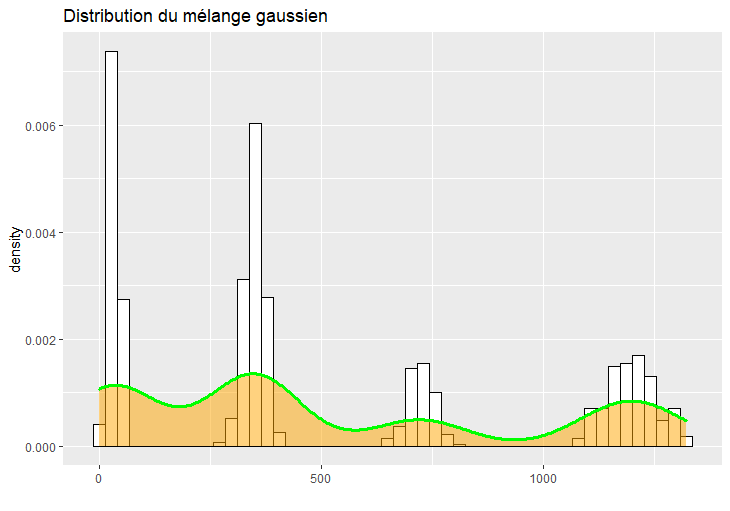
\includegraphics[scale=0.45]{images/dens_sim2.png}
	\caption{Paramètres initiaux choisis}
	\label{density_sim2}
\end{figure}

Nous avons ensuite appliqué notre algorithme (fonction EM) sur cet échantillon. Le tableau \ref{tab3} contient les valeurs des vrais paramètres de ce mélange simulé. Comme il a été mentionné précédemment, le choix des paramètres initiaux est crucial si l'on veut que l'algorithme estime correctement les paramètres du mélange. Le tableau \ref{tab4} contient les valeurs des paramètres initiaux utilisés. Comme vous pouvez le voir en observant ces deux tableaux, nous avons choisi des paramètre initiaux assez proches des vrais de manière à ne pas être bloqué dans des extremas locaux. Les résultats obtenus par notre algorithme sont affichés sur la capture d'écran de la figure \ref{res_sim2}.

Comme on peut le voir sur la figure \ref{res_sim2}, les valeurs estimées par notre implémentation sont proches de celles des vrais paramètres (voir tableau \ref{tab3}). Ces résultats nous montrent conforte une fois de plus dans l'idée que notre fonction $EM$ fonctionne correctement.

\begin{figure}[htp] 
	\centering
	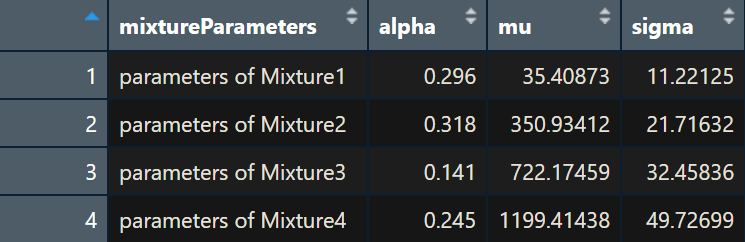
\includegraphics[scale=0.7]{images/res_sim2.png}
	\caption{Paramètres du mélange gaussien estimés par notre fonction $EM$}
	\label{res_sim2}
\end{figure}

\begin{table}[htp]
	\center
	\begin{tabular}{|c||c|c|c|}
		\hline
		& $\alpha$ & $\mu$ & $\sigma$\\
		\hline
		Paramètres du 1er mélange & $0.30$ & $35$ & $11$ \\
		\hline
		Paramètres du 2ème mélange & $0.33$ & $350$ & $22$ \\
		\hline
		Paramètres du 3ème mélange & $0.15$ & $720$ & $32$ \\
		\hline
		Paramètres du 4ème mélange & $0.22$ & $1198$ & $55$ \\
		\hline
	\end{tabular}
	\caption{Vrais paramètres du mélange}
	\label{tab3}
\end{table}

\begin{table}[htp]
	\center
	\begin{tabular}{|c||c|c|c|}
		\hline
		& $\alpha$ & $\mu$ & $\sigma$\\
		\hline
		Paramètres du 1er mélange & $0.33$ & $30$ & $10$ \\
		\hline
		Paramètres du 2ème mélange & $0.30$ & $370$ & $25$ \\
		\hline
		Paramètres du 3ème mélange & $0.17$ & $717$ & $30$ \\
		\hline
		Paramètres du 4ème mélange & $0.20$ & $1238$ & $57$ \\
		\hline
	\end{tabular}
	\caption{Paramètres initiaux choisis}
	\label{tab4}
\end{table}

\newpage

\subsection{Étude sur des données réelles}
Dans cette sous section nous allons appliquer notre algorithme sur des données réelles provenant de la librairies $MASS$. Le jeu de données que nous allons manipuler est celui intitulé $galaxies$. Un extrait du jeu de données est disponible en figure \ref{galaxies}

%\begin{figure}[htp] 
%	\centering
%	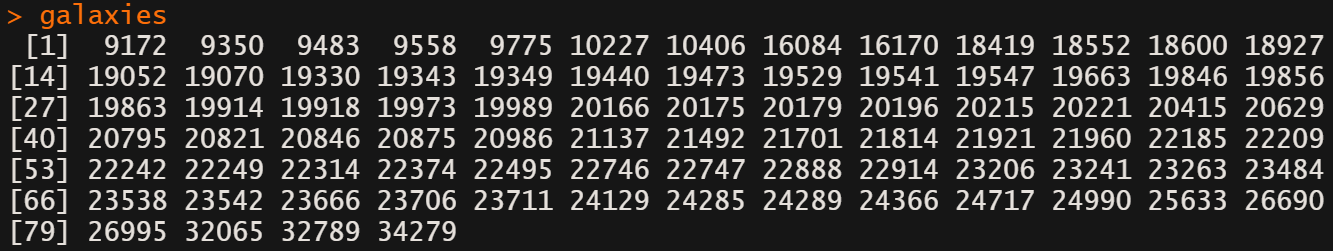
\includegraphics[scale=0.45]{images/dataset.png}
%	\caption{Extrait du jeu de données $galaxies$}
%	\label{galaxies}
%\end{figure}

\newpage

\section{Comparaison de la fonction $EM$ avec $Mclust$}
La librairie $Mclust$ de $R$ est une librairie dans laquelle est implémentée l'algorithme EM. Afin d'evaluer la performance de notre fonction $EM$ nous allons donc la comparer avec celle prédéfini via dans la $Mclust$. Pour cela, nous utiliserons toujours le même jeu de données, à savoir, $galaxies$.

%\begin{figure}[htp] 
%	\centering
%	\subfloat[seuil $\approx 2.7$]{%
%		\includegraphics[scale=0.4]{images/sumBadth.png}%
%	}%
%	\hfill%
%	\subfloat[seuil $\approx 3.65$]{%
%		\includegraphics[scale=0.4]{images/sumGoodth.png}%
%	}%
%	\caption{Résultats donnés en sortie de la fonction \textit{fpot} pour les 2 seuils}
%	\label{summary}
%\end{figure}


%\begin{table}[htp]
%	\center
%	\begin{tabular}{|c||c|c|c|}
%		\hline
%		\diagbox{Niveau de retour}{Périodes ou Années $T$} & $T = 100$ & $T = 500$ & $T = 1000$\\
%		\hline
%		$x_{\frac{1}{T}}$ & $4.686475$ & $4.72502$ & $4.723653$ \\
%		\hline
%	\end{tabular}
%	\caption{Niveaux de retour associés aux périodes de retour $T$}
%	\label{tab3}
%\end{table}

\newpage

\section{Conclusion}
À travers ce projet, nous avons pu voir qu'au fil des années, nous serons confrontés à des valeurs extrêmes de vagues de plus en plus grandes. Cela est sans aucun doute une conséquence de la hausse des températures et en particulier de la montée du niveau des océans. Nous comprenons donc pourquoi la lutte contre le réchauffement climatique est au cœur des enjeux scientifiques actuels. D'autre part, nous avons pu constater que plus nous prendrons des mesures issues de stations proches et plus les données associées à ces dernières seront fortement corrélées. 


\newpage

\section{Annexes}
%Ci dessous, l'export de code permettant d'afficher la liste des diviseurs de $464280$.
%\lstinputlisting[language=R, firstline=19, lastline=26]{code/script_projet_VE_COME_NIASSE.R}

\newpage

\section{Bibliographie}

\renewcommand\refname{}
\begin{thebibliography}{9}
	\bibitem{golfLion}
	\url{https://reporterre.net/Le-golfe-du-Lion-est-tres-vulnerable-a-la-montee-des-eaux}
	page web rédigée par Alexandre Brun et Benoît Devillers
	\bibitem{EM_algorithm}
	Frédéric Santos (2015). L'algorithme EM : une courte présentation
	\url{https://members.loria.fr/moberger/Enseignement/AVR/Exposes/algo-em.pdf}
\end{thebibliography}

\end{document}
